\chapter{Design requirements and architectural choices}
\label{ch:design}


This chapter will discuss multiple architectural design choices to build a Reference Model. This chapter will focus on the overall design and architecture, while \Cref{ch:PipelineShell} and \Cref{ch:ISS} will focus on the pipeline shell and ISS details. Each of these chapters will feature a requirement list for the components. Throughout the following chapters, requirements for the reference model will be indicated with \textbf{RM requirement X}, requirements for the ISS will be indicated with \textbf{ISS requirement X}, and requirements for the pipeline shell will be indicated with \textbf{PS requirement X}. 

\section{Reference Model Requirements}
\label{sec:rm_req}

The main challenges discussed in \cref{sec:back_issProblem} are that when using an ISS as a reference model, asynchronous events can be taken at the wrong time or in the wrong order, and the timing of the side effects can vary between the DUT and the reference model. This happens because the ISS does not have the necessary core-specific pipeline understanding to respond to these asynchronous events correctly.

To overcome these challenges, we should build a reference model that adds a pipeline understanding to the model and use this to time asynchronous events and side effects correctly.

The requirements of the reference model are collected in the requirement list below to concretize the model's development.


\begin{enumerate}
    \item \textbf{The order of the retired instructions should exactly match the core.} \label[rmReq]{rmReq:order}
    \par The order of retired instructions must precisely match the core. This is the fundamental problem the reference model must solve, preventing the issues illustrated in \Cref{fig:lw_example}. This requirement doesn't demand full cycle-accurate simulation but only accurate timing of instructions. While cycle-accurate modeling might be necessary to order instructions correctly with asynchronous events, alternative approaches can be possible. 
    %\par This requirement expresses the main problem the reference model should solve, avoiding problems like the example shown in \Cref{fig:lw_example}. Note that the requirement does not specify full cycle-accurate simulation; only accurate timing of instructions is required. Although cycle-accurate modeling might be required to order instructions correctly with asynchronous events, this also opens up the possibility of other approaches.
    %\item \textbf{The reference model should not allow more state changes than the core } \label[rmReq]{rmReq:}
    %\par This requirement highlights the problem with ImperasDV described in \ref{}.

    \item \textbf{Read the same ELF binary file as the core} \label[rmReq]{rmReq:binary}
    \par The reference model must be able to run the same test program as the core, requiring it to run the same ELF binary file without any modifications to the program or memory map.

    \item \textbf{Output the state changes for comparison at every instruction retirement} \label[rmReq]{rmReq:stateOutput}
    \par To be able to compare the execution of the reference model with the core, we must output the state changes at every instruction retirement. Since the cores in core-v-verif support \acrshort{rvfi} \cite{openhwgroupCorevverifCv32e40sBsp}, we should also output the state changes as \acrshort{rvfi} or \acrshort{rvvi}.

    \item \textbf{Take asynchronous events as inputs independently of the core.} \label[rmReq]{rmReq:asyncInputs}
    \par Interrupts and debug requests should be taken as inputs independently of the core. This avoids the verification hole in \ref{sec:back_issProblem}, where the ISS follows the interrupts the core takes.
    
    \item \textbf{Configurable with the same extensions supported by the core.} \label[rmReq]{rmReq:extensions}
    \par Some cores allow for different extensions to be enabled or disabled. The reference model should also be configurable with different RISC-V extensions to match the core.
    
    \item \textbf{The RM should be as easy to modify to support different cores.} \label[rmReq]{rmReq:modifyable}
    \par Since testbenches shared by multiple cores, like core-v-verif, have become more common, the effort required to modify the reference model for a new core should be as low as possible.
    
   % \item \textbf{Run in lock-step with the core} \label[rmReq]{rmReq:lock-step}
   % \par 
   
   % \item \textbf{Run in the core-v-verif UVM verification environment} \label[rmReq]{rmReq:core-v-verif}
   % \par 

    \item \textbf{Avoid prohibiting support for formal verification} \label[rmReq]{rmReq:formal}
    \par If possible, the reference model should be able to support formal verification. At every design choice, formal verification should be kept in mind.
    
    
\end{enumerate}


\section{Architecture}

As discussed in \Cref{sec:pw_architecture}, the specialization report proposed implementing the reference model with a two-layered modeling technique inspired by the work of \textcite{chiangEfficientTwolayeredCycleaccurate2009} and \textcite{leeFaCSimFastCycleAccurate2008}, which both divided the model into one untimed functional simulator and one timing shell responsible for correctly timing the results generated in the functional simulator. This way, the functional simulator can be general enough to be used by many different cores while all the core-specific functionality is contained in the timing shell.

We choose to implement a similar two-layered division of functionality and timing instead of implementing or modifying a full microarchitectural simulator like gem5 \cite{Gem5Simulator2023} that combines both. This makes configuring the reference model to a new core easier since all the core-specific details should be contained together, fulfilling \Cref{rmReq:modifyable}. 


As discussed in \Cref{sec:pw_architecture}, we can use an existing \acrshort{iss} as the functional simulator and implement the core-specific timing module around it, which we will call the \textit{\gls{ps}} from now on. An ISS steps one instruction at a time and completely finishes all execution of an instruction before moving on to the next. This makes it easy to export a \ccode{step()} function that allows the ISS to do an untimed step, executing one instruction at a time. Since the ISS contains all the functionality, including registers and memory, it must also return the state changes caused by the instruction. This can then be passed to the pipeline shell to time these changes correctly and use them to control the ISS.

The pipelines shell should be responsible \Cref{rmReq:order} and ensure the proper timing and order of retired instructions from the core. It should output the state changes at every instruction retirement (\Cref{rmReq:stateOutput}), giving us \textbf{\Cref{psReq:rvfiOut}}, and correctly time the incoming asynchronous events (\Cref{rmReq:asyncInputs}), giving us \textbf{\Cref{psReq:async_control}}. To do this, it must accurately simulate the pipeline details that are necessary to time asynchronous events, giving us \textbf{\Cref{psReq:pipeline}}. 

\Cref{fig:architecture} shows a block diagram of the proposed architecture for the reference model and relevant surrounding modules. This shows both the pipeline shell and ISS inside the reference model. The test program, interrupts, and debug requests are inserted into the core and pipeline shell, and the RVFI outputs from both are compared in the compare module.

\begin{figure}
    \centering
    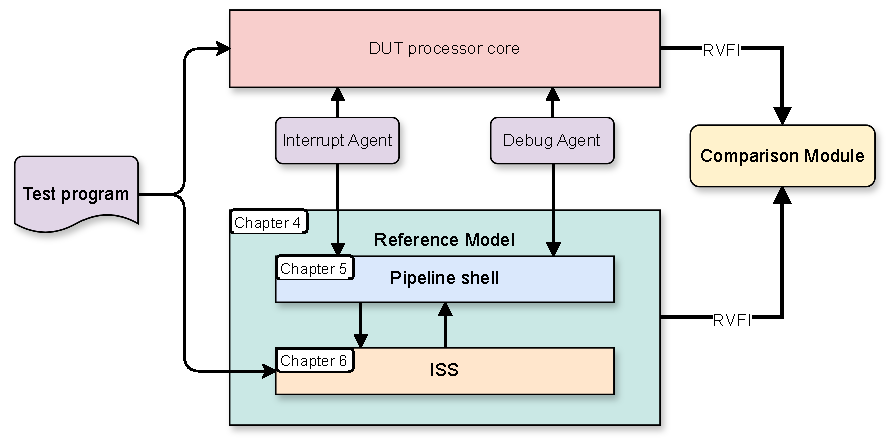
\includegraphics[width=0.75\linewidth]{figures/Architecture.pdf}
    \caption{Block diagram of the reference model architecture.}
    \label{fig:architecture}
\end{figure}

\section{Implementation strategy}
\label{sec:strategy}

We propose the following implementation strategy to build and test the reference model incrementally, ensuring the correct functionality of one phase before moving to the next. This order allows us to develop and verify the simpler, fundamental functionality before using this in the more complex design.

\begin{enumerate}
    \item[\textbf{Phase 1}] Integrate a simple reference model into the testbench, where only the ISS is used. The ISS should step when the core retires an instruction and return RVFI. Normal sequential tests should pass at this phase, but we should disregard asynchronous events. \label{phase:iss}
    \item[\textbf{Phase 2}] Pass interrupts into the reference model in sync with RVFI from the core, resembling traditional ISS simulation from \Cref{sec:bg_iss_refmod}. Interrupt tests should pass. \label{phase:rvfi_interrupt}
    \item[\textbf{Phase 3}] Pass interrupts directly into the reference model asynchronously. Interrupt tests should fail and resemble \Cref{fig:lw_example} since no pipeline shell is implemented.\label{phase:async_fail}
    \item[\textbf{Phase 4}] Develop the pipeline shell to correctly time interrupts. Interrupt tests should pass. \label{phase:pipeline_shell}
\end{enumerate}




\section{Reference Model language}

The core-v-verif verification environment is mainly written in SystemVerilog \cite{openhwgroupOpenhwgroupCorevverif2023}, while many ISSs are written in \cpp or other high-level languages \cite{SpikeRISCVISA2023}.
Therefore, we must decide what language to use to implement the reference model.

To fulfill \textbf{\Cref{rmReq:formal}} and support formal verification, it is best to model the simulator in SystemVerilog to make the reference model synthesizable. This also makes it easier to pass in nets from the rest of the testbench and model parallel components like the pipeline. One disadvantage of using the same language as the core we want to model is that we are more likely to model the reference model similar to the core, potentially modeling the same bugs in both. 

Considering this disadvantage, we still choose to model as much of the reference model as possible in SystemVerilog. 

\section{Reference Model Interface}
\label{sec:rmInterface}

\subsection{RVVI or custom interface}

We can either use RVVI or create our own interface to control the reference model and related testbench components. The RVVI-API is a standard set of API calls meant to decouple the testbench from a specific reference model by abstracting away its details \cite{riscv-verificationRISCVVerificationInterface2023}. 

To comply with \Cref{rmReq:formal}, we want to avoid limiting the possibility of supporting formal verification where this is possible. RVVI is not implemented with formal verification in mind, and there are multiple problems regarding formal verification. One example of this is the \sv{net_push()} and \sv{net_pop()} functions used to pass asynchronous net changes to the reference model, which utilize dynamic arrays. Dynamic arrays are not synthesizable in SystemVerilog \cite{mehtaIntroductionSystemVerilog2021} and are incompatible with formal verification. 

The CV32E40S and other OpenHW cores also support RVFI but not the RVVI-TRACE. Converting the RVFI signals to RVVI-TRACE signals passed to the reference model over the RVVI-API is currently required. 
Although RVVI in itself is open, many of the complimentary components like \sv{trace2cov}, \sv{trace2api}, and \sv{trace2log} are proprietary Imperas components. To use RVVI for our reference model, we would have to model replacements for these components regardless to convert from RVVI-Trace to RVVI-API. 

The design of RVVI also adds some limitations to how the reference model can be built and still support RVVI. Although RVVI is an open standard, it was developed by Imperas and is influenced by the design of ImperasDV. The RVVI-API supports a step-and-compare methodology, where all controls are based on functions. This includes functions for passing the DUT states to the reference model and functions for comparing each state\cite{riscv-verificationRISCVVerificationInterface2023}. As will be discussed further in \ref{sec:des_comparison}, we also want to implement a comparison module that supports assertions, which is complicated by the design of RVVI. 
In \Cref{sec:ps_dependency}, we will also discuss how the reference model should depend on the core. Here, the design of RVVI implicitly restricts our choices. 

To keep our implementation choices independent of RVVI's design and also keep support for formal verification possible, we choose not to support RVVI during the development of the model. Instead, we will make our own interface that can grow to complement the functionality of the reference model. If we discover that the chosen design is compatible with RVVI, support for this can be added in the future, as there are many advantages to using a standardized interface \cite{riscv-verificationRISCVVerificationInterface2023}.


\subsection{Inputs}

To support formal verification, we want to mainly use standard synthesizable signals as inputs and outputs to the reference model instead of communicating with functions. For inputs, we should take the clock and reset signals. To meet \Cref{rmReq:asyncInputs}, the reference model should take the same asynchronous inputs as the core, so we must take the \sv{irq} and \sv{debug_req} signals as inputs. 

Depending on the implementation of the pipeline shell, we also want to inform the reference model every time the core retires an instruction. This is reported from the core through \acrshort{rvfi}, via the \sv{rvfi_valid} signal. The use of this signal will be discussed further in \Cref{sec:ps_dependency}.

To comply with \Cref{rmReq:binary}, we must also input the file path to the test program in the ELF binary file when initializing the reference model. 

%\subsubsection{Binary file}
%In order to fulfill \Cref{rmReq:binary}, we must be able to load an ELF binary file. We therefore need some way of inputting the file path of a binary file into the reference model. In core-v-verif, the path to the binary file is loaded through a command line argument. Since the reference model should run the exact same program, we can read this path inside the reference model wrapper, where we can pass it to the reference model.
%

\subsection{Outputs}

To comply with \Cref{rmReq:stateOutput}, we want to output the state changes for every instruction retirement. Since we decide not to use \acrshort{rvvi}, we choose to output these state changes with \acrshort{rvfi} since the CV32E40S also outputs RVFI, making them easier to compare.

%\subsection{Inputs and outputs}
%
%\begin{itemize}
%    \item IN: clk
%    \item IN: reset
%    \item IN: \sv{irq}
%    \item IN: \sv{debug_req}
%    \item IN: core retirement \sv{rvfi_valid}
%    \item OUT: RVFI
%\end{itemize}


\section{Partitioning between ISS and Pipeline shell}

Having decided to split the functionality between a pipeline shell and an ISS, we must now decide how to partition the functionality between the two components. We can apply general hardware/software functional partitioning principles to achieve this. 
%discusses how \textit{partitioning} of functionality between system components must be chosen to satisfy design constraints and can be used to optimize size/performance, the number of objects, and utilization of hardware/software solutions.
\textcite{gajskiSpecificationDesignEmbedded1994} discusses the \textit{Ratio cut} functional partitioning algorithm, which attempts to minimize the number of intersecting modules between tho groups. We can apply the same principles to achieve a clean partition between the ISS and the pipeline shell.

The specialization project explored three different partitionings and the corresponding interaction between the Pipeline Shell and ISS, described in \Cref{sec:pw_partition}. It concluded with a partition that keeps the ISS intact and minimizes the interactions between the ISS and the pipeline shell. It uses a \sv{step()} function executing one whole instruction and only returns the state changes from this instruction.

We want to fulfill \Cref{rmReq:modifyable} and make the reference model modifiable to different cores. To accomplish this, we should separate core-specific functionality from core-independent functionality. To adhere to the two-layered approach discussed above, we do not want any core-specific details in the ISS, but we still want the ISS to do most of the functional execution. This requires that the pipeline shell is responsible for timing the execution of instructions and asynchronous events in the ISS, giving us \textbf{\Cref{psReq:ISS-control}}. 

Because we want to limit the modifications to the ISS as much as possible, we load the ELF binary file directly into the ISS instead of into the pipeline shell. This gives us \textbf{\Cref{issReq:binaries}}. Additionally, we will use the GPRs, CSRs, PC, and other registers inside the ISS instead of copying them to the pipeline shell. As discussed in \Cref{sec:pw_partition}, using the registers local to the ISS, we also avoid simulating forwarding since all the modifications from an instruction are completed before the next instruction is started. Using the same rationale, we also want to use the memory simulation inside the ISS.

One disadvantage of using the local registers and memory of the ISS is that these can contain some core-specific functionality like memory mapping and imple\-mentation-specific changes to \acrshort{csr}s. This leads to an ISS that is not fully core-independent. To mitigate this, we want to configure these modifications only once at startup, giving us  \textbf{\Cref{issReq:csr}}, stating that the ISS must be configurable to match the core. Because the ISS is responsible for the functional execution of the instructions, it also needs to be configurable to support different RISC-V extensions, as expressed in \textbf{\Cref{rmReq:extensions}}. This gives us \textbf{\Cref{issReq:custom}}. 

Because the ISS is responsible for fetching instructions, executing the instructions, updating registers, and writing to and from memory, this also needs to be reported out of the ISS. We want to use a standard interface to support exchanging the ISS in the future. Since we want to use RVFI as an output of the reference model, it also makes sense to report state changes from the ISS using RVFI. We choose to send RVFI out of the ISS and into the pipeline shell, giving us \textbf{\Cref{issReq:state}} and \textbf{\Cref{psReq:rvfiIn}}.

\Cref{rmReq:asyncInputs} states that the reference model should take asynchronous events as inputs. Since the pipeline shell is responsible for timing asynchronous events, these inputs should also be input into the pipeline shell, giving us \textbf{\Cref{psReq:async_input}}. Since timing asynchronous events rely on core-specific pipeline details, the pipeline shell should control when asynchronous events are taken and inform the ISS when to take these, giving us \textbf{\Cref{psReq:async_control}} and \textbf{\Cref{psReq:ISS-control}}.

\section{ISS Interface}

Since we want to keep as much of the core functionality in the pipeline shell as possible, the ISS should be as generic as possible. With this distinct separation between the pipeline shell and the ISS, we should also make the ISS easily replaceable. This gives us \textbf{\Cref{issReq:replacable}}. 

To make the ISS replaceable, we should create an ISS wrapper with generic functions called by the rest of the reference model. This way, the underlying ISS in the wrapper can be replaced without replacing the functions in the rest of the reference model.
We can use functions to interact with the ISS from the reference model since these work with RTL code and C/\cpp over \acrfull{dpi} (\Cref{sec:bg_dpi}). Functions do not consume time in SystemVerilog \cite{mehtaIntroductionSystemVerilog2021}, so using these to control the ISS ensures that the ISS remains functional and that only the pipeline shell is responsible for timing.

We need to implement the following functions to control the ISS, but the specifics will be discussed in \Cref{ch:ISS}.

\begin{itemize}
    \item \sv{iss_init(...)} - Load ELF binary file and configure the ISS.
    \item \sv{iss_step(...)} - Step through one instruction and return state changes (RVFI)
    \item \sv{iss_intr(...)} - Inform of asynchronous interrupts
    \item \sv{iss_debug(...)} - Inform of asynchronous debug requests
\end{itemize}




\section{Supporting Formal Verification}

\Cref{rmReq:formal} states that, if possible, support for formal verification should not be hindered. Formal verification has many benefits compared to simulation, as discussed in \Cref{sec:bg_formal}, so a future goal is to have a complete reference model compatible with formal verification.

A reference model that is synthesizable and compatible with formal verification can also be compatible with traditional simulation. It would be a very powerful tool if the reference model could be built to support both formal verification and simulation.

Sequential \acrfull{fev} is a formal method comparing two RTL models over time. This has the possibility of working with a reference model, but it requires all the outputs of the core and reference model matches for every cycle \cite{seligmanFormalVerificationEssential2015}.

A simpler approach without using \acrfull{fev} is described in \Cref{sec:bg_eq_abv}, where  \acrfull{sva} are used to compare the core and reference model. Because we only need to compare the core and reference model at instruction retirements, we do not need the two to be equal for every cycle. Instead, we can define a set of assertions that compare each RVFI output between the core and reference models when an instruction retires. Using assertions in the comparison module, these can be used both for formal and simulation-based verification \cite{seligmanFormalVerificationEssential2015}.

\subsection{Synthesisable RTL}

Most available tools for formal verification require that both the implementation and specification models be synthesizable \acrshort{rtl} blocks \cite{seligmanFormalVerificationEssential2015}. This is a significant disadvantage compared to traditional simulation testbenches, since it would not be possible to use \acrshort{dpi} functions to integrate an ISSs written in \cpp into the model. This drastically limits the available ISSs since most are written in \cpp or other languages. Because of this, we set formal verification support as an optional requirement in \textbf{\Cref{issReq:formal}}.

Considering the pipeline shell, this should be possible to make compatible with formal verification, so the whole reference model is compatible with formal verification if a "formal friendly" ISS is used. This gives us \textbf{\Cref{psReq:formal}}.


\section{Testbench Architecture}
\label{sec:testbench}


The current implementation of core-v-verif uses ImperasDV as a reference model. ImperasDV is a \acrfull{vip} that also handles the comparison between the \acrshort{dut} and reference model \cite{imperassoftwareltdRISCVProcessorOVP2023}. To replace ImperasDV with the reference model, we must also implement a comparison module to compare the core with the reference model. This section will cover the integration of the reference model into the larger \gls{core-v-verif} testbench and the design of the comparison module used to compare the core and reference model.

The spike version recently added to core-v-verif has a corresponding RVFI agent and scoreboard used to tie Spike to the rest of core-v-verif and compare the core to Spike. One solution could be to integrate the reference module with these components. These rely on non-synthesizable SystemVerilog functionality \cite{mehtaIntroductionSystemVerilog2021} like classes and UVM. To fulfill \Cref{rmReq:formal} and support formal verification, we can not use these constructs and have to make our own comparison module and interface with the reference model that is compatible with formal verification.


\subsection{Comparison module}
\label{sec:des_comparison}

\subsubsection{Compare at retirement or clock}
\label{sec:des_retireOrClock}

When comparing the reference model to the core, we have some choices about when to do so. One solution is to ensure that both are equal at every clock cycle, while the standard approach for other step-and-compare methodologies is to compare the two only when an instruction retires.

Generally, we want to keep the reference model's abstraction level as high as possible. 

When verifying that the processor adheres to the RISC-V ISA specification, the critical thing is that the order and correctness of instructions are correct, not necessarily the exact cycle this happens on. By comparing the reference model and the core only on instruction retirements, we also give the reference model some slack and the possibility of operating on a higher abstraction layer. This is useful to avoid implementing the same bugs in the reference model and the core.

We choose to compare the reference model and core at every instruction retirement.

%\subsubsection{Timing differences between the core and reference model}
%
%If retirements from the core drive the reference model, as will be discussed in \Cref{sec:ps_dependency}, this has some implications on the timing between them.
%
%The reference module requires the \sv{rvfi_valid} signal from the core to determine when to step the reference model.
%
%
%If we pass the same clock into both, the valid signal out of the core will be one cycle delayed into the reference model as shown in \Cref{fig:1clocktiming}. When comparing the two, we have to delay the core RVFI signals, so they arrive at the compare module simultaneously or use \sv{\$past()} to compare the RM with the previous cycle of the core. We choose to delay the RVFI output from the core one cycle.
%
%\begin{figure}
%    \centering
%    \begin{tikztimingtable}
%      \sv{clk}    & G   6{4C} G \\ % ends with edge
%      \sv{rvfi_core.valid}  & 4L 8H 12L \\
%      \sv{rvfi_core}        & 4U 8D{N} 12U \\
%      \sv{rvfi_rm.valid}    & 2H 10L 8H 4L \\
%      \sv{rvfi_rm}          & 2D{N-1} 10U 8D{N} 4U \\
%    \end{tikztimingtable}
%    \caption{Timing diagram showing the \sv{rvfi_valid} signals of the core and reference model when the reference model is dependent on retirements from the core.}
%    \label{fig:1clocktiming}
%\end{figure}


\subsubsection{Assertions}

To support formal verification, we use \acrfull{sva} to compare the reference model and the core to achieve equivalence checking using \acrfull{abv}, explained in \Cref{sec:bg_eq_abv}. \acrshort{sva} can also be used for simulation and formal verification, making the same comparison module usable for simulation and formal verification \cite{cernySVAPowerAssertions2015}. 

%From \Cref{fig:2clocktiming} we see that if we sampled at the rising edge of \sv{rvfi_rm.clk} shown in red, we would sample the old value of \sv{rvfi_rm.valid} and the signals would not be equal. To fix this we can sample at a point where both signals are equal at the beginning of the simulation step, which is the case for the falling edge of \sv{rvfi_rm.clk}, the falling edge of \sv{rvfi_core.clk} or the rising edge of \sv{rvfi_core.clk}. 

Concurrent assertions use sampled values from the beginning of the simulation step \cite{cernySVAPowerAssertions2015}. 
If we compare the two at the rising edge of \sv{rvfi_core.clk} we can check the correctness using a \acrshort{sva} shown in \Cref{lst:pc_assertion}. 

To only compare the core and \acrshort{rm} at instruction retirements, we check if \sv{rvfi_rm.valid} is high in the antecedent, before comparing the \sv{pc_rdata} signals in the consequent. This structure can be applied to all the \acrshort{rvfi} signals.

As will be discussed in \Cref{sec:ps_dependency}, the reference model is dependent on instruction retirements from the core, delaying the reference model one cycle behind the core. To use the assertion from \Cref{lst:pc_assertion}, we must delay the RVFI output from the core one cycle.

\begin{systemverilog}[caption={Assertion comparing the PC of the \acrshort{rm} and core.}, label={lst:pc_assertion}]
rvfi_pc_a: assert property( @(posedge rvfi_core.clk)
    rvfi_rm.valid |-> (rvfi_rm.pc_rdata == rvfi_core.pc_rdata));
\end{systemverilog}




\subsection{Integration with core-v-verif}

To include the reference model into core-v-verif, we make a wrapper module called \file{uvmt_cv32e40s_reference_model_wrap.sv}. The wrapper instantiates the reference and comparison modules and takes in the RVFI output from the core, interrupts from the interrupt agent, and debug requests from the debug agent. It passes the clock and reset, \rv{rvfi_valid}, \rv{irq}, and \rv{debug_req} into the reference model.

It also passes the RVFI output of the core and reference model into the comparison module, which compares the two.



%
%Another solution is to use two separate clocks for the core and reference model. By having the clock of the reference model slightly offset behind the clock of the core, we get the timing diagram shown in \Cref{fig:2clocktiming} with the two clocks \sv{rvfi_core.clk} and \sv{rvfi_rm.clk} for the core and reference model, the two valid signals \sv{rvfi_core.valid} and \sv{rvfi_rm.valid}, and the rest of the rvfi signals. Here we see that the signals are equal for most of the time, and by comparing at the right clock edge, we can directly compare the equality of the signals. The lines in \Cref{fig:2clocktiming} show different clock edges we can use to compare the signals.
%
%
%\tmp{How does this work with formal verification?}
%
%using the \lstinline{set_clock_spec} with \lstinline{--pulse_offset time}  in onespin we can add multiple clocks. \cite{onespin_reference_manual?} 
%
%\tmp{TODO: test dette}
%
%
%
%\par\bigskip
%% Vurder å bruke wavedrom
%%{signal: [
%%  {name: 'core.clk', wave: 'p....', period: 2},
%%  {name: 'rm.clk', wave: 'P...', period:2, phase: -0.5},
%%  {name: 'core.valid', wave: '0.10.', period: 2},
%%  {name: 'rm.valid', wave: '0.10.', period: 2, phase: -0.5},
%%], head:{
%%   text:'WaveDrom example',
%%   tick:0,
%%   every:2,
%%  	
%%   }
%%  }
%\begin{figure}
%    \centering
%    \begin{tikztimingtable}
%      \sv{rvfi_core.clk}      & [C] 5{4C} C \\ % starts with edge
%      \sv{rvfi_rm.clk}      & LL   5{4C} G \\ % ends with edge
%      \sv{rvfi_core.valid}  & G 8L 8H 8L \\
%      \sv{rvfi_core}  & G 8U 8D{N} 8U \\
%      \sv{rvfi_rm.valid}    & 2H 8L 8H 6L \\
%      \sv{rvfi_rm}    & 2D{N-1} 8U 8D{N} 6U \\
%    \extracode
%        \vertlines[red]{10}
%        \vertlines[green]{14}
%        \vertlines[blue]{16}
%    %\extracode
%    %  \tablerules
%    %  \begin{pgfonlayer}{background}
%    %    \foreach \n in {1,...,8}
%    %      \draw [help lines] (A\n) -- (B\n);
%    %  \end{pgfonlayer}
%    \end{tikztimingtable}
%    \caption{Timing diagram with a seperate offset clock for the reference model and the valid signals for the core and reference model.}
%    \label{fig:2clocktiming}
%\end{figure}
%


